\documentclass[12pt,a4paper]{article} %12 кегль, формат бумаги А4, тип статья

\usepackage[T2A]{fontenc} %поддержка кириллицы
\usepackage[utf8]{inputenc} %кодировка символов юникод
\usepackage[english,russian]{babel} %список рабочих языков
\usepackage{cmap} %для поиска в pdf
\usepackage[left=2cm,right=2cm,top=2cm,bottom=2cm]{geometry} %размеры отступов от краев страницы
\usepackage{graphicx} %возможность работать с графикой
\usepackage{enumitem} %для работы со списками
\usepackage{float} %для точного размещения таблиц и графики
\usepackage{caption} %для создания подписей таблиц и графики
\usepackage{amsmath,amssymb,amsthm,amsfonts} %штуки для математики
\usepackage{extarrows} %чтобы подписи над и под нестандартными стрелками писать короче в коде
\usepackage{makeidx} %собирает ключевые слова для предметного указателя
\usepackage[hidelinks]{hyperref} %убирает выделение ссылок; добавляет гиперссылки в оглавление, перекрестные ссылки и URL
\usepackage{setspace} %устанавливает отступы
\linespread{1.5} %длина межстрочного интервала
\vspace{125mm} %длина абзацного отступа
\usepackage{titlesec}
\titleformat{\section}{\normalfont\Large\bfseries\centering}{}{0pt}{} % эти две строчки убирают циферки перед названиями разделов в основном тексте и выравнивают названия секций по центру
\usepackage{paratype} %чтобы точно был поиск и шрифт хороший

\author{Автор конспекта: Краснов Б. А.}
\title{Запорожец Д.Н.: Случайные блуждания и процессы Леви}
\date{весна 2026}

\newtheorem{theorem}{Теорема}
\newtheorem{lemma}{Лемма}
\newtheorem{definition}{Определение}
\newtheorem{proposition}{Предложение}
\newtheorem{consequence}{Следствие}
\newcommand{\R}{\mathbb{R}}
\newcommand{\Co}{\mathbb{C}}
\newcommand{\E}{\mathbb{E}}
\newcommand{\D}{\mathbb{D}}
\newcommand{\PR}{\mathbb{P}}
\newcommand{\charf}[2][\lambda]{\varphi_{#2}(#1)}
\newcommand{\F}{\mathcal{F}}
\newcommand{\M}{\mathfrak{M}}

\begin{document}
	\maketitle
	\tableofcontents
	\clearpage
	\section{Одномерное случайное блуждание}
	\subsection{1-й закон арксинуса}
	\begin{definition}
		Пусть $\{\xi_i\}_{i=1}^{n}-i.i.d.\in\R$. Тогда будем называть $\{S_i\}_{k=0}^{n}$-случайное блуждание, где 
		$S_0=0,S_k=\displaystyle\sum_{i=1}^k\xi_i$.
	\end{definition}
	\begin{theorem}
		(Sparre Anderson, 1949). Пусть $\{S_i\}_{k=0}^{n}$-случайное блуждание удовлетворяющее следующим условиям:
		\begin{enumerate}
			\item (GP) $\PR(S_k=0)=0$;
			\item (Sym) $\xi_k\overset{d}{=}-\xi_k$.
		\end{enumerate}
		Тогда $\PR(S_1>0,\cdots S_n>0)=\displaystyle\frac{(2n-1)!!}{(2n)!!}$.
	\end{theorem}
	\begin{proof}
		Во-первых, максимум случайного блуждания в каждой реализации единственный, так как в противном случае разность между ними нарушала бы условие (GP).
		\begin{figure}[H]
			\centering
			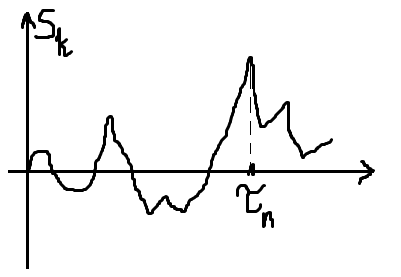
\includegraphics{max_time_S_k.png}
			\caption{Точка максимума блуждания}
		\end{figure}
		Обозначим за $\tau_n: S_{\tau_n}=\underset{k\in\overline{0,n}}{\max}\{S_k\}$. Зафиксируем $k\in\overline{0,n}$. Тогда получаем:
		$$\PR(\tau_n=k)=\PR(S_k>S_{k-1},\cdots,S_k>S_0,S_k>S_{k+1},\cdots,S_k>S_n)=$$
		$$=\PR(\xi_k>0,\cdots,\sum_{i=1}^k\xi_i>0,\xi_{k+1}<0,\cdots,\sum_{i=k+1}^n\xi_i<0)$$
		Нетрудно видеть, что внутри вероятности событие, отвечающее двум реализациям независимых случайных блужданий, а именно $\PR(\cdot)=p_k p_{n-k}$, где $p_k=\PR(S_1>0,\cdots,S_k>0)$. Далее немного поиграем с производящими функциями:
		$$1=\sum_{k=0}^n\PR(\tau_n=k)=\sum_{k=0}^np_k p_{n-k}$$
		$$x^n=\sum_{k=0}^np_k p_{n-k}x^k\quad|x|<1$$
		$$\frac{1}{\sqrt{1-x}}=\left(\sum_{n=0}^{+\infty}p_n x^n\right)$$
		$$(1+y)^{\alpha}=\sum_{n=0}^{+\infty}\binom{n}{\alpha}y^n\quad y=-x, \alpha=-\frac{1}{2}$$
	\end{proof}
	\begin{consequence}\label{т_момент максмимума симRWG}
		(Дискретный закон Sparre Anderson). $\PR(\tau_n=k)=\displaystyle\frac{(2k-1)!!}{(2k)!!}\cdot\displaystyle\frac{(2n-2k-1)!!}{(2n-2k)!!}$
	\end{consequence}
	\begin{consequence}
		Тождество Чжу-Вандермонда: $\displaystyle\sum_{k=0}^n\binom{2k}{k}\binom{2n-2k}{n-k}=2^{2n}$
	\end{consequence}
	%док-во Болотин
	\begin{proof}
		Чисто комбинаторного доказательства за несколько часов найдено не было.
	\end{proof}
	\begin{consequence}
		$p_n=\displaystyle\frac{1+o(1)}{\sqrt{\pi n}}\quad n\rightarrow +\infty$
	\end{consequence}
	\begin{proof}
		Формула Стирлинга:
		$$\frac{(2n-1)!!}{(2n)!!}=\frac{(2n)!}{(2^nn!)^2}=(1+o(1))\frac{\sqrt{2\pi n}\left(\frac{2n}{e}\right)^{2n}}{2\pi n\left(2^n\left(\frac{n}{e}\right)^n\right)^2}=(1+o(1))\frac{1}{\sqrt{\pi n}}$$
	\end{proof}
	\begin{consequence}
		$\lim\limits_{n\rightarrow +\infty}\PR\left(\displaystyle\frac{\tau_n}{n}\leq t\right)=\frac{2}{\pi}\arcsin\sqrt{t}=\frac{1}{\pi}\displaystyle\int_0^t\frac{ds}{\sqrt{s(1-s)}}$
	\end{consequence}
	\begin{proof}
		Мы хотим найти предельное значение следующей величины:
		$$\PR\left(\frac{\tau_n}{n}\leq t\right)=\lim\limits_{n\rightarrow +\infty}\sum_{k=0}^{[nt]}\PR\left(\frac{\tau_n}{n}=\frac{k}{n}\right)=\lim\limits_{n\rightarrow +\infty}\sum_{k=0}^{[nt]}p_kp_{n-k}=\lim\limits_{n\rightarrow +\infty}\sum_{\left\{k\vert\,\, 0\leq\frac{k}{n}\leq t\right\}}p_kp_{n-k}$$
		Из предыдущего следствия мы знаем предельное значение $p_n$, но нам нужно стремление индексируемого множителя к бесконечности. Давайте пока будем считать, что $t\geq \frac{1}{2}$, тем самым сможем оценить хвостовое значение верхнего ряда, так как в этом случае выполнено:
		$$\frac{1}{2}\leq\frac{k}{n}\leq t\Rightarrow n,n-k\rightarrow +\infty\,\, \emph{при}\,\,n\rightarrow +\infty$$
		Тогда вспоминая предыдущую лемму и определение интеграла Римана получаем:
		$$\sum_{\left\{k\vert\,\, \frac{1}{2}\leq\frac{k}{n}\leq t\right\}}p_kp_{n-k}=(1+o(1))\cdot\sum_{\left\{k\vert\,\, \frac{1}{2}\leq\frac{k}{n}\leq t\right\}}\frac{1}{\pi}\frac{1}{\sqrt{k(n-k)}}=$$
		$$=(1+o(1))\cdot\sum_{\left\{k\vert\,\, \frac{1}{2}\leq\frac{k}{n}\leq t\right\}}\frac{1}{n\pi}\frac{1}{\sqrt{\frac{k}{n}(1-\frac{k}{n})}}=\frac{1}{\pi}\int_{\frac{1}{2}}^t\frac{ds}{\sqrt{s(1-s)}}$$
		Теперь, как нетрудно заметить, под интегралом стоит симметричная функция на отрезке $[0,1]$ относительно вертикальной прямой $x=\frac{1}{2}$, являющаяся плотностью распределения максимума блуждания (с точностью до нормировочного коэффициента), а также очевидно, что если в исходной теореме взять $t=\frac{1}{2}$, то получим значение $\frac{1}{2}$. Тем самым теорема верна для $t\geq \frac{1}{2}$, а тогда из симметричности и замены переменной в интеграле для всех $t\in [0,1]$.
	\end{proof}
	\subsection{Перестановочные случайные блуждания}
	\begin{definition}
		Случайные величины $\{\xi_i\}_{i=1}^n$ называются перестановочными, если:
		$$\forall\sigma\in Sym_n\quad (\xi_1,\cdots,\xi_n)\overset{d}{=}\sigma(\xi_1,\cdots,\xi_n)$$
	\end{definition}
	Примеры:
	\begin{enumerate}
		\item i.i.d.;
		\item Равномерное распределение на сфере;
		\item Пусть есть уран с m белыми шарами и n черными. Будем реализовывать случайную выборку без возвращения и определим случайные величины $\xi_k=1$, если k шар черный и 0 иначе.
	\end{enumerate}
	\begin{definition}
		Пусть $\{\xi_k\}_{k=0}^n$ перестановочны. Тогда $\{S_k\}_{k=0}^n, S_0=0, S_k=\displaystyle\sum_{i=1}^k\xi_i$ перестановочное случайное блуждание.
	\end{definition}
	Пример: $\{\xi_k\}_{k=1}^n-i.i.d.\Rightarrow Y_k=\xi_k-\displaystyle\frac{S_n}{n}$ перестановочное блуждание.
	\begin{definition}
		Перестановочное случайное блуждание называется случайным мостом, если $\PR(S_n=0)=1$.
	\end{definition}
	\begin{theorem}
		(Sparre Anderson, 1949). Пусть $\{S_k\}_{k=0}^n$ случайный мост с условием\\ $\PR(S_k=0)=0,k\in \overline{1,n-1}$. Тогда $\PR(S_1,\cdots,S_{n-1}>0)=\displaystyle\frac{1}{n}$.
	\end{theorem}
	\begin{proof}
		Используя перестановочность получаем следующую цепочку равенств:
		$$\PR(\xi_1>0,\xi_1+\xi_2>0,\cdots,\xi_1+\cdots+\xi_{n-1}>0)=$$
		$$=\PR(\xi_2>0,\xi_2+\xi_3>0,\cdots,\xi_2+\cdots+\xi_n>0)=\cdots$$
		$$=\PR(\xi_n>0,\xi_n+\xi_1>0,\cdots,\xi+n+\xi_1+\cdots+\xi_{n-1}>0)$$
		Возьмем произвольную реализацию нашего случайного моста и посмотрим на графики траекторий, сдвигая последовательность шагов частицы на один по циклу. Заметим, что тогда только одна траектория будет все время не ниже нуля: существование - так как можем начать из самой нижней точки исходной траектории, единственность - если есть две нижнее точки в исходной траектории и хотя бы одна из них не начало и не конец, то тогда нарущается условие, которое мы наложили на случайный мост.
		\begin{figure}[H]
			\centering
			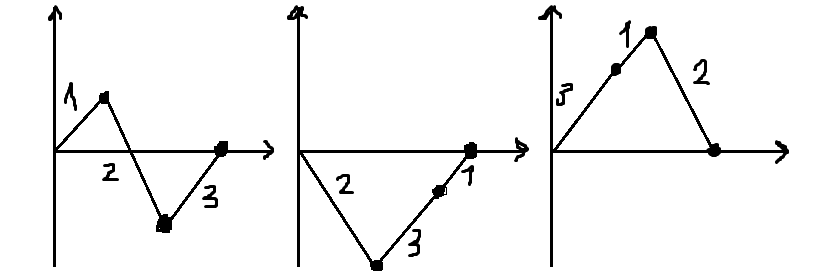
\includegraphics{track_prob_bridge.png}
			\caption{Пример для трех величин}
		\end{figure}
		Тем самым каждую вероятность в цепочке равенств можно понимать так: правда ли, что при зафиксированных значениях $\xi_k$, если бы начали ходить так, то получится траектория не ниже 0. Тогда все вероятности в цепочке равенств дизъюнктны и составляют полную вероятность, а значит каждая равна $\displaystyle\frac{1}{n}$.
	\end{proof}
	\begin{definition}
		Пусть $\{S_k\}_{k=0}^n$ перестоновочное случайное блуждание. Положим за $\tau_n$ момент первого максимума блуждания; $\alpha_n=\#\{k\in\overline{1,n}\vert S_k>0\}$.
	\end{definition}
	\begin{theorem}\label{о числе пол. моментов ERBG}
		Пусть $\{S_k\}_{k=0}^n$ случайный мост с условием $\PR(S_k=0)=0,k\in \overline{1,n-1}$. Тогда $\PR(\alpha_n=k)=\displaystyle\frac{1}{n},k\in\overline{0,n-1}$.
	\end{theorem}
	\begin{proof}
		Действовать будем аналогично доказательству предыдущей теоремы. Возьмем произвольную реализацию блуждания и будем по циклу переставлять величины, порождающие блуждание. Заметим, что из условия (GP) следует, что (п.н.) среди $\{S_k\}_{k=0}^{n-1}$ нет двух равных, а тогда для фиксированной реализации блуждания, ставя 0 блуждания в разные места получим разные значения $\alpha_n$. Проще это понять на картинке: продлим блуждание на одну копию вправо, тогда все вершины на разных высотах и значит над каждой горизонтальной прямой, выпущенной из вершин $\{S_k\}_{k=0}^{n-1}$, разное число точек блуждания, от 0 до n.
		\begin{figure}[H]
			\centering
			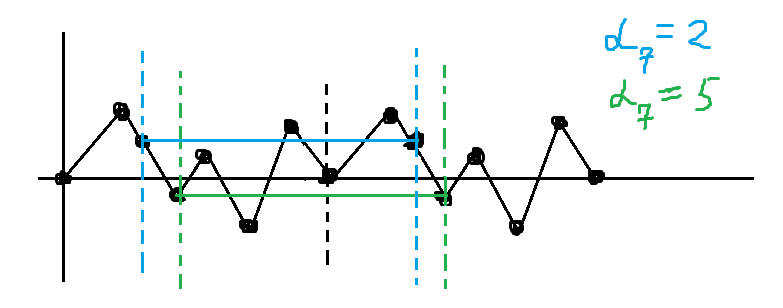
\includegraphics{ERBG_alpha.png}
			\caption{Поясняющий пример}
		\end{figure}
		Раз величины перестановочны и каждая реализация циклическим сдвигом порождает все значения $\alpha_n$, то все значения принимаются с равной вероятностью.
	\end{proof}
	\begin{consequence}
		Пусть $\{S_k\}_{k=0}^n$ случайный мост с условием $\PR(S_k=0)=0,k\in \overline{1,n-1}$. Тогда $\tau_n\overset{d}{=}\alpha_{n}$
	\end{consequence}
	\begin{proof}
		Снова действуем также, как в теореме выше. Пусть при исходной реализации $\tau_n=k$, тогда при сдвиге на 1 по той же картинке вправо значение $\tau_n$ упадет на 1. Так происходит до мометна, когда максимум станет началом блуждания и $\tau_n=0$ соответсвенно. При следующем сдвиги максимум станет равен n и далее снова падать на 1.
	\end{proof}
	\begin{theorem}\label{о распр максимума ERWG}
		Пусть $\{S_k\}_{k=0}^n$ перестоновочное случайное блуждание с условием (GP), тогда $\tau_n\overset{d}{=}\alpha_{n}\overset{d}{=}U(\overline{0,n})$.
	\end{theorem}
	\begin{proof}
		Положим $S_{n+1}\equiv0$. Это не случайная величина, поэтому вероятностная структура не портится и таким действием мы превращаем исходное ERWG на n вершинах в ERBG на n+1 вершине. Заметим, что при любой реализации блуждания при этом преобразовании значения $\tau_n,\alpha_n$ не меняются, а их распределения для ERBG на n+1 вершине мы знаем из предыдущего следствия.
	\end{proof}
	Введем несколько обозначений для наших конструкций.
	% вообще во всей этой истории хочется примеров и по возможности простых и по возможности в непрерывном и дискретном случае
	\begin{enumerate}
		\item RW - класс случайных блужданий (i.i.d.);
		\item ERW - класс перестановочных случайных юлужданий;
		\item RWG - класс случаных блужданий с условием (GP);
		\item ERWG - перестановочные случайные блуждания с условием (GP);
		\item ERB - мосты;
		\item ERBG - мосты с условием (GP).
	\end{enumerate}
	\subsection{Геометрический пример моста в $\R^2$}
	Обозначим за $\mathcal{F}_k(P)$ - множество k-мерных граней многоугольника P в $\R^d$.
	\begin{theorem}
		Пусть $\{S_k\}_{k=0}^n$ - ERWG в $\R^2$. Тогда:
		$$\E|\mathcal{F}_1(conv(S_0,\cdots,S_n)|=2H_n$$
	\end{theorem}
	\begin{proof}
		\,\\Замечание: условие (GP) означает, что $\forall k\in\overline{1,n-1}\,\,\forall 1\leq j_1\leq\cdots\leq j_k\leq n\,\, S_{j_1},\cdots,S_{j_k}$ линейно независимы с вероятностью 1.\\
		Если посмотреть на выпуклую оболочку нашего блуждания, то ее стороны это отрезки с концами в каких-то $S_k$ и на внутренности сторон (п.н.) нет никаких $S_k$. Тогда можно сделать следующие нехитрые преобразования:
		$$\E|\mathcal{F}_1(conv(S_0,\cdots,S_n)|=\E\sum_{0\leq k<l\leq n}I_{\{[S_k,S_l] - \emph{сторона выпуклой оболочки}\}}=$$
		$$=\sum_{0\leq k<l\leq n}\PR([S_k,S_l] - \emph{сторона выпуклой оболочки})=\sum_{j=1}^n\sum_{i=0}^{n-j}\PR([S_i,S_{i+j}] - \emph{сторона выпуклой оболочки})$$
		Теперь посчитаем отдельно каждую вероятность в этой сумме. Общая идея такова: мы рассмотрим случайную прямую, проходящую через $S_i,S_{i+j}$, от которой в наших рассуждениях для конструкции блуждания потребуется только угол наклона прямой, который задается вектором $S_{i+j}-S_i$, то есть зависит от $\{\xi_l\}_{l=i}^{i+j}$; далее берем ортогональную прямую к этой и проецируем блуждание на нее (более точно поворачиваем прямую на угол $\frac{-\pi}{2}$, направление у нас уже есть, а 0 будет проекция 0); спроецированное блуждание будет состоять из трех частей: два ERWG и ERBG постоянного знака и пользуясь перестановочностью получаем, что два ERWG можно объеденить в одно у которого максимум должен быть в момент $i$, а тогда вероятность уже легко вычислить по ранее полученным результатам.
		\begin{figure}[H]
			\centering
			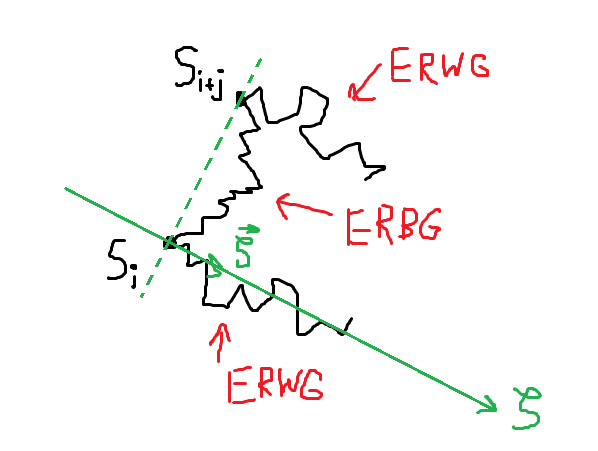
\includegraphics{convex_ERWG.png}
			\caption{геометрический взгляд}
		\end{figure}
		Итак, положим за $\overrightarrow{\zeta}:=(S_{i+j}-S_i)^{\bot}$ случайный вектор с направлением как на картинке выше, а за $\zeta$ обозначим координатную прямую вдоль этого вектора с началом в $S_i$, тогда каждая отдельная вероятность равна:
		$$\PR([S_i,S_{i+j}] - \emph{сторона выпуклой оболочки})=\PR([\overrightarrow{\eta},S_l-S_i] > 0,\,l\in\overline{0,n}\setminus\overline{i,i+j};\,\{\xi_k\}_{k=i+1}^{i+j} - ERBG)=$$
		$$=\PR([\overrightarrow{\eta},S_l-S_i] > 0,\,l\in\overline{0,n}\setminus\overline{i,i+j}\mid\{\xi_k\}_{k=i+1}^{i+j} - ERBG)\cdot\PR(\{\xi_k\}_{k=i+1}^{i+j} - ERBG)\boxed{=}$$
		Далее воспользуемся перестановочностью, а именно:
		$$(\xi_1,\cdots,\xi_i,\xi_{i+1},\cdots,\xi_{i+j},\xi_{i+j+1},\cdots,\xi_n)\overset{d}{=}(\xi_1,\cdots,\xi_i,\xi_{i+j+1},\cdots,\xi_n,\xi_{i+1},\cdots,\xi_{i+j})$$
		То есть переставим величины порождающие мост в конец. Переобозначим величины и введем новые одномерные:
		$$(\xi_1,\cdots,\xi_i,\xi_{i+j+1},\cdots,\xi_n,\xi_{i+1},\cdots,\xi_{i+j})=:(\widehat{\xi}_1,\cdots,\widehat{\xi}_i,\widehat{\xi}_{i+1},\cdots,\widehat{\xi}_{n-j},\widehat{\xi}_{n-j+1},\cdots,\widehat{\xi}_n)$$
		$$\eta_i:=Pr_{\zeta}(\widehat{\xi}_i+S_i)$$
		Тогда вероятность, которую мы хотим посчитать равна:
		$$\boxed{=}\PR(\{\eta_k\}_{k=1}^{n-j} - ERWG\,\emph{с максимумом в}\,\, i\mid\{\widehat{\xi}_k\}_{k=n-j+1}^{n} - ERBG)\cdot\PR(\{\widehat{\xi}_k\}_{k=n-j+1}^{n} - ERBG)$$
		Теперь заметим, что события в условной вероятности не зависят друг от друга, а значит условная вероятность просто равна событию, что максимум блуждания в момент i. Тогда применяя утверждения\eqref{о распр максимума ERWG},\eqref{о числе пол. моментов ERBG} получаем:
		$$\PR([S_i,S_{i+j}] - \emph{сторона выпуклой оболочки})=\frac{1}{n-j+1}\cdot\frac{1}{j}$$
		Теперь заметим, что ввиду однозначного выбора направления $\eta$ мы упустили случай, когда вся конструкция по другую сторону прямой, тем самым:
		$$\E|\mathcal{F}_1(conv(S_0,\cdots,S_n)|=\sum_{j=1}^n\sum_{i=0}^{n-j}\frac{2}{j(n-j+1)}=2H_n$$
		Замечание: внезапные прибавления $S_i$ выше, это переход из одной системы координат в другую. Также не трудно понять, что условие главной позиции сохраняется при проецировании блуждания на любую прямую.
	\end{proof}
	\subsection{Второй закон арксинуса (Sparre Anderson)}
	\begin{theorem}
		Пусть $\{S_k\}_{k=0}^n$ - ERW, $\tau_n$ - момент первого максимума:\\ $S_0,\cdots,S_{\tau_n-1}<S_{\tau_n}\geq S_{\tau_n+1},\cdots,S_n$, $\alpha_n=\#\{k\in\overline{1, n}\vert S_k>0\}$. Тогда $\alpha_n\overset{d}{=}\tau_n$.
	\end{theorem}
	\begin{consequence}
		Если $\{S_k\}_{k=0}^n$ - симметричное RWG (как в самой первой теореме), то
		$$\PR(\alpha_n=k)=\frac{1}{2^{2n}}\binom{2k}{k}\binom{2n-2k}{n-k}$$
	\end{consequence}
	\begin{proof}
		Вспомнить чему равно распределение момента максимума при таком блуждании\eqref{т_момент максмимума симRWG}.
	\end{proof}
	\begin{consequence}
		Пусть $W_t,\,t\in[0,1]$ - броуновское движение. Тогда случайная величина $\displaystyle\int_0^1I_{\{W_t>0\}}(t)dt$ имеет плотность $\displaystyle\frac{2}{\pi}\cdot\frac{1}{\sqrt{s(1-s)}}$
	\end{consequence}
	\begin{proof}
		%Лиза
	\end{proof}
	Сформулируем комбинаторную лемму, которая поможет доказать вероятностное утверждение. Пусть дан набор вещественных чисел $\{x_i\}_{i=1}^n$, тогда для произвольной $\sigma\in Sym_n$ положим
	$$s_k(\sigma):=\sum_{i=1}^kx_{\sigma(i)}$$
	\begin{lemma}
		Для произвольного набора вещественных чисел $\{x_i\}_{i=1}^n$ и для произвольного числа $r\in\overline{0,n}$ верно следующее:
		$$\#\{\sigma\in Sym_n\mid\sum_{k=0}^nI_{\{s_k(\sigma)>0\}}=r\}=\#\{\sigma\in Sym_n\mid s_0(\sigma)\cdots s_{r-1}(\sigma)<s_r(\sigma)\geq s_{r+1}(\sigma)\cdots s_n(\sigma)\}$$
	\end{lemma}
	Теперь за бесплатно докажем теорему.
	\begin{proof}
		В качетсве набора чисел ясное делое используем реализации величин образающих блуждание.
		$$\PR(\alpha_n=r)=\PR\left(\sum_{k=0}^nI_{\{S_k>0\}}=r\right)\overset{\emph{перестановочность}}{=}\frac{1}{n!}\sum_{\sigma\in Sym_n}\PR\left(\sum_{k=0}^nI_{\{s_k(\sigma)>0\}}=r\right)=$$
		$$=\frac{1}{n!}\E\sum_{\sigma\in Sym_n}I_{\left\{\sum_{k=0}^nI_{\{s_k(\sigma)>0\}}=r\right\}}\overset{\emph{лемма}}{=}\frac{1}{n!}\E\sum_{\sigma\in Sym_n}I_{\{s_0(\sigma)\cdots s_{r-1}(\sigma)<s_r(\sigma)\geq s_{r+1}(\sigma)\cdots s_n(\sigma)\}}=$$
		$$=\frac{1}{n!}\sum_{\sigma\in Sym_n}\PR\left(s_0(\sigma)\cdots s_{r-1}(\sigma)<s_r(\sigma)\geq s_{r+1}(\sigma)\cdots s_n(\sigma)\right)\overset{\emph{перестановочность}}{=}$$
		$$=\PR(S_0\cdots S_{r-1}<S_r\geq S_{r+1}\cdots S_n)=\PR(\tau_n=r)$$
	\end{proof}
	Теперь докажем саму лемму.
	\begin{proof}
		%дописать
	\end{proof}
	\subsection{Формула Спицера (Spitzer)}
	Обозначим значения максимума и минимума блуждания: $\overline{S_n}:=S_{\tau_n},\,\underline{S_n}:=\min(S_0,\cdots,S_n)$
	\begin{theorem}
		Пусть $\{S_k\}_{k=0}^{+\infty}$ - RW. Тогда при $|t|<1,\,Im\,\lambda\geq0$ имеем:
		$$\sum_{n=0}^{+\infty}t^n\E e^{i\lambda\overline{S_n}}=\exp\left\{\sum_{n=1}^{+\infty}\frac{t^n}{n}\E e^{i\lambda S_n^{+}}\right\}$$
	\end{theorem}
	\begin{consequence}
		(Кац, 1954) $\E\overline{S_n}=\displaystyle\sum_{k=1}^n\frac{1}{k}\E S_k^{+}$
	\end{consequence}
	\begin{proof}
		Положим $\lambda=ix$ и возьмем производную по x в формуле Спицера (почленное диффиринцирование возможно, так как все сходится абсолютно и равномерно ввиду выбора t).
		$$\frac{d}{dx}\left(\sum_{n=0}^{+\infty}t^n\E e^{-x\overline{S_n}}\right)=-\sum_{n=0}^{+\infty}t^n\E\overline{S_n}e^{-x\overline{S_n}}$$
		$$\frac{d}{dx}\left(\exp\left\{\sum_{n=1}^{+\infty}\frac{t^n}{n}\E e^{-x S_n^{+}}\right\}\right)=-\exp\left\{\sum_{n=1}^{+\infty}\frac{t^n}{n}\E e^{i\lambda S_n^{+}}\right\}\cdot\sum_{n=1}^{+\infty}\frac{t^n}{n}\E S_n^{+}e^{-x S_n^{+}}$$
		Подставляя x=0, получаем:
		$$\sum_{n=0}^{+\infty}t^n\E\overline{S_n}=\frac{1}{1-t}\sum_{n=1}^{+\infty}\frac{t^n}{n}\E S_n^{+}=\sum_{n=0}^{+\infty}t^n\cdot\sum_{n=1}^{+\infty}\frac{t^n}{n}\E S_n^{+}$$
		Тогда коэффициенты перед $t^n$ в обоих частях равны и дают нам нужное тождество.
	\end{proof}
	\begin{consequence}
		$$\E(\overline{S_n}-\underline{S_n})=\sum_{k=1}^n\frac{1}{k}\E|S_k|$$
	\end{consequence}
	\begin{proof}
		Нетрудно видеть, что если заменить $\xi\mapsto-\xi$, то тогда \\$\overline{S_n}\mapsto\underline{S_n},\,S_n^{+}\mapsto S_n^{-}$, а также $\E S_k^{+}-\E S_k^{-}=\E|S_k|$
	\end{proof}
	\begin{consequence}
		(Обобщение т. Sparre Anderson)
		$$\sum_{n=0}^{+\infty}t^n\PR(S_1,\cdots,S_n\geq0)=\exp\left\{\sum_{n=1}^{+\infty}\frac{t^n}{n}\PR(S_n\geq0)\right\}$$
	\end{consequence}
	\begin{proof}
		Снова положим $\lambda=ix$ и заметим, что если $\xi$ неотрицательная случайная величина, то верно:
		$$\lim\limits_{x\rightarrow+\infty}\E e^{-x\xi}=\PR(\xi=0)$$
		Тогда из формулы Спицера получаем (заметим, что $\overline{S_n}$ неотрицательна ввиду $S_0=0$):
		$$\sum_{n=0}^{+\infty}t^n\PR(S_1,\cdots,S_n\leq0)=\sum_{n=0}^{+\infty}t^n\PR(\overline{S_n}=0)=\lim\limits_{x\rightarrow+\infty}\sum_{n=0}^{+\infty}t^n\E e^{-x\overline{S_n}}=$$
		$$=\lim\limits_{x\rightarrow+\infty}\exp\left\{\sum_{n=1}^{+\infty}\frac{t^n}{n}\E e^{-x S_n^{+}}\right\}=\exp\left\{\sum_{n=1}^{+\infty}\frac{t^n}{n}\PR(S_n\leq0)\right\}$$
		Для получение требуемого результат снова заменяем все случайные величины на противоположные.
	\end{proof}
	Обозначим за $c_k(\sigma)$ количество циклов в $\sigma$ длины k. Заметим, что $\displaystyle\sum_{k=1}^nkc_k(\sigma)=n$.
	\begin{lemma}
		$$\#\{\sigma\in Sym_n\mid c_k(\sigma)=i_k,\,k\in\overline{1,n}\}=\frac{n!}{\prod_{k=1}^nk^{i_k}i_k!}$$
	\end{lemma}
	\begin{proof}
		Пусть нам дан набор чисел $\{l_k\}_{k=1}^m:1\leq l_k\leq n,\,l_1+\cdots+l_m=n$ и мы хотим составить все перестановки длины $n$, которые раскладываются в произведение циклов с длинами $l_k$. Не трудно понять, что число способов разбить $n$ чисел на нужные группы нужного размера равно:
		$$C=\prod_{k=1}^m\binom{n-s_k}{l_k}=\frac{n!}{\prod_{k=1}^ml_k!},\quad s_k:=\sum_{i=1}^{k-1}l_i$$
		Теперь заметим, что из $l_k$ чисел можно составить $(l_k-1)!$ цикл. Также циклы коммутируют друг с другом, а значит если $l_i=l_j$, то выбирая сначала элементы первого цикла, а потом другого мы посчитали одну и ту же перестановку несколько раз. Тем самым искомый ответ равен:
		$$\frac{n!}{\prod_{k=1}^ml_k!}\cdot\prod_{k=1}^m(l_k-1)!\prod\frac{1}{\prod_{k=1}^mc_k!},\quad c_k=\#\{l_i:l_i=k\}$$
		Что в точности совпадает с утверждением леммы, если заменить переменные. (Простите за излишнюю строгость)
	\end{proof}
	\begin{consequence}
		$$\sum_{\substack{i_1,\cdots,i_n\geq0 \\ i_1+\cdots+ni_n=n}}\frac{1}{\prod_{k=1}^nk^{i_k}i_k!}=1$$
	\end{consequence}
	\begin{lemma}
		Пусть есть вещественная аналитичная в 0 функция с положительным радиусом сходимости и рядом $\displaystyle\sum_{n=0}^{+\infty}a_nt^n$. Тогда в круге сходимости верно:
		$$\exp\left\{\sum_{n=0}^{+\infty}a_nt^n\right\}=\sum_{n=0}^{+\infty}t^n\left(\sum_{i_1+\cdots+ni_n=n}\prod_{k=1}^n\frac{a_k^{i_k}}{i_k!}\right)$$
	\end{lemma}
	\begin{proof}
		%что-то не сходится со свободным членом
	\end{proof}
	Теперь преступим к доказательсту формулы Спицера.
	\begin{proof}
		%дописать
	\end{proof}
	\subsection{Факторизация Винера-Хопфа}
	%дописать
	\subsection{Возвратность случайного блуждания}
	\begin{definition}
		Пусть $(\Omega,\mathcal{F},\PR)$ - вероятностное пространство. Фильтрацией называется последовательность возрастающих под-$\sigma$-алгебр $\mathcal{F}_n\subset\mathcal{F}$ (у нас будет дискретное время, то есть индексы натуральные). Если дана последовательность случайных величин $\{\xi_k\}_{k=1}^{+\infty}$, то естественной фильтрацией, порожденной этими величинами называется последовательность из следующих $\sigma$-алгебр: $\mathcal{F}_n=\sigma\{\xi_1,\cdots,\xi_n\}$
	\end{definition}
	\begin{definition}
		Случайная величина $\tau:\Omega\rightarrow\mathbb{N}$ называется моментом остановки относительно фильтрации $\{\mathcal{F}_n\}_{n=1}^{+\infty}$, если $\forall n\in\mathbb{N}:\{\tau\leq n\}\in\mathcal{F}_n$
	\end{definition}
	\begin{theorem}
		(Первое тождество Вальда) Пусть $\{\xi_n\}_{n=1}^{+\infty}$-i.i.d.; $\E|\xi_1|<+\infty$; $\tau$ - момент остановки относительно естественной фильтрации: $\E\tau<+\infty$, тогда выполнено:
		$$\E|S_{\tau}|<+\infty,\quad\E S_{\tau}=\E\xi_1\cdot\E\tau,\quad S_k:=\sum_{i=1}^k\xi_i$$
	\end{theorem}
	\begin{proof}
		$$\E|S_{\tau}|=\E\E(|S_{\tau}|\mid\tau)=\E\sum_{k=1}^{+\infty}\E(|S_{\tau}|\mid\tau=k)I_{\{\tau=k\}}\leq\E\sum_{k=1}^{+\infty}k\E|\xi_1|I_{\{\tau=k\}}=\E|\xi_1|\cdot\E\tau$$
		Тем самым конечность показали $S_{\tau}\in L^1$, а равенство получаем также, только убираются модули и знак с неравенства переходит в равенство.
	\end{proof}
	Замечание: мне не совсем понятно зачем накладывать условие конечности мат. ожидания на момент остановки, разве что только для того, чтобы обе части равенства были конечны, но вроде доказательству это не протеворечит, а в литературе и интернете я комментария к этому не нашел. Принадлежность $\xi_1\in L^1$ существенна, так как иначе просто не определено мат. ожидание от частичных сумм.
	\section{Процессы Леви}
	\subsection{Предварительные сведения}
	Поговорим сначала о естественном обобщении случайного блуждания. Изначально у нас каждую единицу времени происходил один шаг блуждания. Далее логично рассматривать ситуации, в которых время между шагами случайно. В связи с этим можно ввести слудующие конструктивные определения:
	\begin{definition}
		Пусть $\{\xi_n\}\in\R^d$-i.i.d. величины, тогда за $N(t)$ определим простой пуассоновский процесс, как:
		$$N(t):=\inf\{n\mid\sum_{k=1}^n\eta_k>t\},\quad\{\eta_n\}\in\R-i.i.d.;\,\eta_1\overset{d}{=}Exp(\lambda)$$
		А за $S(t)$ обозначим сложный пуассоновский процесс:
		$$S(t):=\sum_{k=1}^{N(t)}\xi_k$$
	\end{definition}
	Сделаем следующее замечание: для удобства будем считать, что $\xi_n\in E:=\R^d\setminus\{0\}$, то есть насильно уберем существования атома, который переводится в 0.
	\begin{definition}
		Топологическое пространство называется польским, если существует на нем метрика, которая порождает его топологию, в которой оно полно и сепарабельно.
	\end{definition}
	\begin{enumerate}
		\item $\R^n$;
		\item сепарабельные банаховы или гильбертовые пространства;
		\item метрические компакты;
		\item $C[0,1]$
		\item $\R^n\setminus\{0\}$  с метрикой $d(x,y):=|x-y|+||x|^{-1}-|y|^{-1}|$
	\end{enumerate}
	\begin{definition}
		Пусть $E$ произвольное польское пространство с борелевской $\sigma$-алгеброй $\mathcal{B}(E)$. Обозначим за $M(E)$ множество локально конечных мер на $(E,\mathcal{B}(E))$, то есть таких, что для каждой точки есть окрестность с конечной мерой. Тогда можно ввести на $M(E)$ $\sigma$-алгебру: это будет минимальная $\sigma$-алгебра $\M(E)$, такая что для любого \\$B\in\mathcal{B}(E)$ отображение $f_B:M(E)\rightarrow\R:\mu\mapsto\mu(B)$ измеримо, где на $\R$ стандартная $\sigma$-алгебра.
	\end{definition}
	\begin{definition}
		Пусть $(\Omega,\F,\PR)$ вероятностное пространство, тогда случайный элемент $\xi:\Omega\rightarrow M(E)$ будем называть случайной локально конечной мерой (точнее его реализацию).
	\end{definition}
	\begin{definition}
		Случайная локально конечная мера, принимающая неотрицательные целые значения называется случайным точечным процессом.
	\end{definition}
	\begin{definition}
		Случайный точечный процесс $N_{\mu}$ называется пуассоновским точечным процессом на $E$ с интенсивностью $\mu\in M(E)$, если:
		\begin{enumerate}
			\item Для любого $B\in\mathcal{B}(E)$ и любого $k\in\{0,1,\cdots\}$ верно:
			\begin{equation*}
				\PR(N_{\mu}(B)=k)=
				\begin{cases}
					\frac{\mu(B)^k}{k!}e^{-\mu(B)},\,\,\mu(B)<+\infty \\
					0,\,\,\mu(B)=+\infty
				\end{cases}
			\end{equation*}
			\item Для любых дизъюнктных множеств $B_1,\cdots,B_n\in\mathcal{B}(E)$ случайные величины $N_{\mu}(B_1),\cdots,N_{\mu}(B_n)$ независимы.
		\end{enumerate}
	\end{definition}
	
	Теперь посмотрим на конструктивное построение данного процесса. Заранее скажем, что всю конструкцию можно обобщить и на пространства с $\sigma$-конечной мерой, просто представив пространство ввиде дизъюнктного объединения подпространств с конечной мерой, а вероятностным пространством будет произведение соответсвующих конструкций.
	
	Рассмотрим произвольное измеримое пространство $(E,\mathcal{E},\mu)$ с конечной мерой. Введем пуассоновскую случайную величину $\eta$ с параметром $\mu(E)$, которая отвечает за число выделенных точек в пространстве. Отнормировав меру пространства мы получаем вероятностную меру: $\PR(A)=\displaystyle\frac{\mu (A\cap E)}{\mu (E)}\quad \forall A\in \mathcal{E}.$ Введем случайную величину $\xi$, которая будет иметь распределение $\PR (\xi \in A)=\displaystyle\frac{\mu (A\cap E)}{\mu (E)}$, а ее реализациями будут особые точки пространства.
	
	Разыграем $\eta$ и определим пространство конфигураций $R_\eta = \{\xi_{1},\xi_{2},...,\xi_{\eta}\}$, где \\ 
	$\forall i=\overline{1,\eta}\quad \xi_{i} \stackrel{d}{=} \xi$ и они независимы в совокупности. Теперь определим 
	случайную меру следующим образом: $\forall A\in \mathcal{E} \quad \nu (A) := \# A\cap R_\eta$. Несложно доказать, что это действительно пуассоновский точечный процесс:
	\begin{theorem}	
		\,
		\begin{enumerate}
			\item $\forall A\in \mathcal{E} \quad \nu (A) \stackrel{d}{=} \mathrm{P}(\mu (A))$;
			\item $\forall A_{1},...A_{n} \in \mathcal{E}-\emph{дизъюнктных}\Rightarrow \nu (A_{1}),...,\nu (A_{n})-\emph{независимы в совокупности}$.
		\end{enumerate}
	\end{theorem}
	\begin{proof}
		\,
		\begin{enumerate}
			\item Прямыми вычислениями получаем:
			$$\PR (\nu (A)=k) = \sum_{n=0}^{+\infty}\PR (\nu (A)=k\mid \eta =n)\PR (\eta =n) = $$ 
			$$= \sum_{n=k}^{+\infty}\binom{n}{k}\frac{\mu (A)^{k}[\mu (E)-\mu (A)]^{n-k}}{\mu (E)^{n}} e^{-\mu (E)}\frac{\mu (E)^{n}}{n!} 
			= e^{-\mu (A)}\frac{\mu (A)^{k}}{k!}$$
			\item Так как множества дизъюнктны, то реализация каждой случайной величины может вносить вклад не более чем в одно множество, откуда следует тривиальная проверка независимости по определению:
			$$\PR (\nu (A_{1}=a_{1}),...,\nu (A_{n}=a_{n})) = \sum_{s=0}^{+\infty}\PR (\nu (A_{1}=a_{1}),...,\nu (A_{n}=a_{n})\mid \eta =s)\PR (\eta =s) = $$
			$$= \sum_{s=N}^{+\infty}\left[ e^{-\mu (E)}\frac{\mu (E)^{s}}{s!} \binom{s}{a_{1},...,a_{n},s-N} \prod_{i=1}^{n}\left(\frac{\mu (A_{i})}{\mu (E)}\right)^{a_{i}} \frac{(\mu (E)-\mu (\bigcup_{j=1}^{n}A_{j}))^{s-N}}{\mu (E)^{s-N}}\right]=$$
			$$=e^{-\mu (E)}\prod_{i=1}^{n}\frac{\mu (A_{i})^{a_{i}}}{a_{i}!}\sum_{s=0}^{+\infty}\frac{(\mu (E)-\mu (\bigcup_{j=1}^{n}A_{j}))^{s}}{s!}=\prod_{i=1}^{n}\PR (\nu (A_{i})=a_{i}),$$
			где $N=\displaystyle\sum_{i=1}^{n}a_{i}$
		\end{enumerate}
	\end{proof}
	Пусть $f:X\rightarrow \R$ измеримая функция.
	\begin{definition}
		Стохастическим интегралом $f$ будем называть $$\int\limits_{E}fd\nu := \sum_{\xi \in R_{\eta}}f(\xi)$$ иногда 
		сокращая обозначение до $F$.
	\end{definition}
	\begin{proposition}
		\label{prop1}
		Для стохастическего интеграла $f$ верны следующие утверждения
		\begin{enumerate}
			\item $\E F= \displaystyle\int\limits_Efd\mu$ если $f\in L^1 (\mu)$;
			\item $\D F= \displaystyle\int\limits_Ef^2d\mu$ если $f\in L^2 (\mu)$;
			\item $\charf{F}=\exp\left(\displaystyle\int\limits_E(e^{itf}-1)d\mu\right)$.
		\end{enumerate}
	\end{proposition}
	\begin{proof}
		Расписывая математическое ожидание через интеграл получаем следующее равенство:
		\begin{equation*}
			\E f^p(\xi)=\frac{1}{\mu (E)^p}\displaystyle\int\limits_Ef^pd\mu \quad \forall p\in \mathbb{N}
		\end{equation*}
		и его следствие:
		\begin{equation*}
			\D f(\xi)=\frac{1}{\mu (E)}\displaystyle\int\limits_Ef^2d\mu - \frac{1}{\mu (E)^2}\left(\displaystyle\int\limits_Efd\mu\right)^2
		\end{equation*}
		Теперь используя эти равенства и тождество Вальда немедленно получаем первые два пункта леммы.
		Также можно было доказать эти утверждения несложным вычислением через условное математическое ожидание, как мы это сделаем для подсчета характеристической функции.
		$$\charf{F}=\E\E (e^{itF}\vert \eta)=\sum_{n=0}^{+\infty}\PR (\eta =n)(\charf{f(\xi)})^n =\exp\left(\displaystyle\int\limits_E(e^{itf}-1)d\mu\right)$$
	\end{proof}
	Теперь можно представить сложный пуассоновский процесс как:
	$$S(t)=\int\limits_{\R\times E}xI_{[0,t]}(s)N_{\mu}(ds,dx),$$
	где $N_{\mu}$ пуассоновский точечный процесс на $\R_{\geq0}\times E$ с мерой интенсивности $\mu=\lambda\cdot ds\times\nu$, где $\nu$ - распределение $\xi_1$
	\subsection{Процессы Леви и разложение Леви-Ито}
	\begin{definition}
		Процесс $\xi(t)$ в $\R^d$ называется процессом Леви, если выполнены следующие условия:
		\begin{enumerate}
			\item $\xi(0)=0$ п.н.;
			\item независимость приращений: $\forall0\leq t_1<\cdots<t_n\,\,\xi(t_1),\xi(t_2)-\xi(t_1),\cdots,\xi(t_n)-\xi(t_{n-1})$ независимы;
			\item стационарность приращений: $\xi(t+s)-\xi(s)\overset{d}{=}\xi(t)$
			\item стохастическая непрерывность: $\lim\limits_{h\rightarrow0}\xi(t+h)\overset{\PR}{=}\xi(t)$
		\end{enumerate}
	\end{definition}
	Известна следующая теорема, доказываемая, например, в основном курсе ТВ:
	\begin{theorem}
		(Представление Леви-Хинчина) Пусть $\xi\in\R^d$ - случайный вектор с хар. функцией $\charf{\xi}$. Тогда $\xi$ безгранично делим (представляется в виде произвольной конечной суммы i.i.d. величин) тогда и только тогда, когда существуют $a\in\R^d,\,Q\in\R^{d\times d}$ - симметричная неотрицательно определенная матрица и мера Леви $\mu$ на $E=\R^d\setminus\{0\}$ такие что выполнены:
		$$\int\limits_E\min(1,x^2)\mu(dx)<+\infty$$
		$$\charf{\xi}=\exp\left\{i\langle\lambda,a\rangle-\frac{1}{2}\langle\lambda,Q\lambda\rangle+\int\limits_E(e^{i\langle\lambda,x\rangle}-1-i\langle\lambda,x\rangle I_{\{|x|\leq1\}}(x))\mu(dx)\right\}$$
	\end{theorem}
	Тогда нетрудно видеть, что если $\xi$ процесс Леви, то $\xi(t)$ безгранична делима:
	$$\xi(t)=\sum_{k=1}^n\xi\left(\frac{kt}{n}\right)-\xi\left(\frac{(k-1)t}{n}\right)$$
	И тогда из того же представления получаем тройку Леви - $(a,Q,\mu)$, характеризующую процесс:
	$$\log\charf{\xi(1)}=i\langle\lambda,a\rangle-\frac{1}{2}\langle\lambda,Q\lambda\rangle+\int\limits_E(e^{i\langle\lambda,x\rangle}-1-i\langle\lambda,x\rangle I_{\{|x|\leq1\}}(x))\mu(dx)$$
	Рассмотрим в качестве примера сложный пуассоновский процесс. Пусть экспоненциальные величины из его определения имеют параметр $\alpha$, тогда имеем $\PR(N(t)=n)=\frac{(t\alpha)^n}{n!}e^{-t\alpha}$, откуда нетрудно получить представление его хар. функции:
	$$\charf{S(t)}=e^{t\alpha(\charf{\xi_1}-1)}$$
	\begin{lemma}
		Пусть $\xi$ процесс Леви, тогда для любого $\lambda\in\R^d$ следующее отображение непрерывно:
		$$t\mapsto\charf{\xi(t)}=\E e^{i\langle\lambda,\xi(t)\rangle}$$
	\end{lemma}
	\begin{proof}
		Для произвольного $\varepsilon>0\,\exists\delta_1>0:$
		$$|e^{i\langle\lambda,x\rangle}-1|<\varepsilon,\quad\emph{при}\,|x|<\delta_1$$
		А из стохастической непрерывности $\exists\delta_2>0$:
		$$\PR(|\xi(t)-\xi(s)|>\delta_1)<\varepsilon,\quad\emph{при}\,|t-s|<\delta_2$$
		Тогда получаем оценку:
		$$|\E e^{i\langle\lambda,\xi(t)\rangle}-\E e^{i\langle\lambda,\xi(s)\rangle}|\leq\{\emph{выносим общий множитель и оцениваем из независимости 1}\}\leq$$
		$$\leq|\E e^{i\langle\lambda,\xi(t)-\xi(s)\rangle}-1|\leq\E|e^{i\langle\lambda,\xi(t)-\xi(s)\rangle}-1|I_{\{|\xi(t)-\xi(s)|>\delta_1\}}+\E|e^{i\langle\lambda,\xi(t)-\xi(s)\rangle}-1|I_{\{|\xi(t)-\xi(s)|\leq\delta_1\}}\leq2\varepsilon+\varepsilon$$
	\end{proof}
	\begin{theorem}
		Пусть $\xi$ процесс Леви, тогда $\charf{\xi(t)}=e^{t\log\charf{\xi(1)}}$.
	\end{theorem}
	\begin{proof}
		Из независимости и стационарности приращений получаем мультипликативность хар. функции процесса (просто расписать через мат. ожидание хар. функции), а из непрерывности отображения $t\mapsto\charf{\xi(t)}$ получаем, что это отображение есть экспонента, а начальное значение в 1 нам известно.
	\end{proof}
	\begin{consequence}
		Распределение процесса Леви $\xi$ полностью определяется распределением $\xi(1)$.
	\end{consequence}
	\begin{proof}
		$$\PR(\xi(t_1)\in B_1,\cdots,\xi(t_n)\in B_n)=\PR(\sum_{i=1}^k\xi(t_i)-\xi(t_{i-1})\in B_k,\,k\in\overline{1,n},t_0=0)=$$
		$$=\int\limits_{\R^{d\times n}}\prod_{k=1}^nI_{\{x_1+\cdots+x_k\in B_k\}}\mu(dx_1)\cdots\mu(dx_n),$$
		где $\mu(dx_k)$ - распределение $\xi(t_k)-\xi(t_{k-1})\overset{d}{=}\xi(t_k-t_{k-1})$ - выражается через $\charf{\xi(1)}$
	\end{proof}
	\begin{theorem}
		(Разложение Леви-Ито) Пусть даны $a\in\R^d,Q\in\R^{d\times d},\mu$ - мера Леви на $E$. Тогда существует процесс Леви $\xi$ с тройкой Леви $(a,Q,\mu)$.
	\end{theorem}
	\begin{proof}
		Пусть $rk\,Q=m$, тогда рассмотрим $\sqrt{Q}\in\R^{d\times m}:Q=\sqrt{Q}\sqrt{Q}^T$ и пусть $W(t)$ стандартный винеровский процесс в $R^m$.
		
		Тогда процесс $\xi_1(t):=\sqrt{Q}W(t)+ta$ является процессом Леви и имеет экспоненту Леви:
		$$\log\charf{\xi_1(1)}=i\langle\lambda,a\rangle-\frac{1}{2}\langle\lambda,Q\lambda\rangle$$
		Рассмотрим $N$ - пуассоновский точечный процесс на $\R_{+}\times E$ с мерой интенсивностью $dt\times\mu$ и рассмотрим
		$$\xi_2(t)=\int\limits_{\R_{+}\times E\setminus\{|x|\leq1\}}xN(ds,dx)I_{[0,t]}$$
		Тогда получаем:
		$$\log\charf{\xi_2(1)}=t\int\limits_{E\setminus\{|x|\leq1\}}(e^{i\langle\lambda,x\rangle}-1)\mu(dx)$$
		Осталось разобраться с происходящим в единичном шаре. Заметим, что сразу по нему проинтегрировать мы не могли ввиду расходимости интеграла, согласно т. Кемпбелла. В таком случае расмматривают в единичном шаре не просто пуассоновскую меру, а ее центрированную версию.
		$$\xi_3(t)=\int\limits_{[0,t]\times\{x:|x|<1\}}x\{N(ds,dx)-\E N(ds,dx)\}=\int\limits_{[0,t]\times\{x:|x|<1\}}x\{N(ds,dx)-ds\times\mu(dx)\}$$
		Таким образом требуемый процесс Леви с нужной тройкой будет суммой
		$$\xi(t)=\xi_1(t)+\xi_2(t)+\xi_3(t)$$
	\end{proof}
	\subsection{Примеры и следствия из разложения Леви-Ито}
	Посмотрим на представления Леви (логарифм хар. функции $\xi(1)$ через тройку Леви) известных процессов. Для стандартного винеровского процесса $W(t)$ разложение много раз встречалось: $\psi(\lambda)=-\frac{1}{2}\lambda^2$. Также не сложно вычислить представление для сложного пуассоновского процесса:
	$$\psi(\lambda)=\alpha(\varphi(\lambda)-1)=\alpha\left(\int\limits_E(e^{i\langle\lambda,x\rangle}-1)\nu(dx)\right)=$$
	$$=i\langle\lambda,a\rangle+\int\limits_E(e^{i\langle\lambda,x\rangle}-1-i\langle\lambda,x\rangle I_{\{x:|x|<1\}})\mu(dx)$$
	где $\mu=\alpha\nu,\,a=\int\limits_{|x|<1}x\mu(dx)$
	\begin{definition}
		Процесс Леви $\xi\in\R$ называется субординатором, если он имеет неубывающую модификацию п.н.
	\end{definition}
	Таким например является пуассоновский процесс.
	\begin{theorem}
		Процесс Леви с тройкой $(a,Q,\mu)$ является субординатором тогда и только тогда, когда
		$$Q=0,\,\mu((-\infty,0))=0,\,\int_0^1x\mu(dx)<+\infty,\,a_0:=a-\int_0^1x\mu(dx\geq0$$
	\end{theorem}
	\subsection{Траектории процессов Леви}
	\begin{definition}
		Пусть $(E,d)$ метрическое пространство, тогда функция $f:[0,T]\rightarrow E$ называется cadlag если она всюду непрерывна справа и имеет всюду левосторонние пределы (обозначим их $f(t-)$).
	\end{definition}
	\begin{lemma}
		Если $f:[0,T]\rightarrow \R^d$ - cadlag, то она ограничена и имеет не более счетного числа точек разрыва.
	\end{lemma}
	\begin{proof}
		Ограниченность: пусть нет, тогда есть последовательность $\{t_n\}$, что $f(t_n)\rightarrow\infty$. Возьмем сходящуюся монотонную подпоследовательность $\{t_{n_k}\}:t_{n_k}\rightarrow t$. Это можно сделать, например построив конструктивно по пикам. Точка $t_n$ называется пиком соответсвующей последовательности, если для любого $k>n$ выполнено $t_k<t_n$. Если пиков бесконечно, то они подходят, если их конечное число, тогда берем последний пик, далее точку, которая не ниже него, далее точку которая не ниже этой и так далее. Далее из них можно выбрать сходящуюся подпоследовательность из компактности отрезка.
		
		Есть два случая. Либо $t_{n_k}\uparrow t$, но тогда получаем противоречие с существованием левостороннего предела (он должен быть конечен), либо $t_{n_k}\downarrow t$, но тогда противоречие с непрерывностью справа.
		
		Определим $A_m=\{t:|f(t)-f(t-)|\geq\frac{1}{m}\}$. Покажем конечность $A_m$, откуда последует вторая часть леммы.
		
		Снова возьмем сходящуюся монотонную последовательность и далее в зависимости от типа монотонности получаем противоречие с условиями cadlag.
	\end{proof}
	\begin{lemma}
		Равномерный предел cadlag функций есть cadlag функции (естественно все на одном отрезке задано).
	\end{lemma}
	\begin{proof}
		Просто упражнение с кванторами и $\varepsilon-\delta$ формализмом, ну или если более "культурно", то надо использовать $\varepsilon/3$ прием.
	\end{proof}
	Пусть $Z(t)$, где $t\in[0,T]$, случайный одномерный процесс, который имеет п.н. непрерывную справа модификацию $\widehat{Z}(t)$. Тогда %дописать
\end{document}